\chapter{Git}
\label{sec:ch3}
% Old Ch. 3

Git is important because it allows you to work and communicate with people by using just a few simple commands. By following its rules and conventions, you can work with others efficiently, without having to send zip files back and forth through emails. It also allows version control, for you to keep track of changes you have made to your code, and revert to a previous version or take reference from your previous changes when necessary.
\vspace{6mm}

We will focus on getting Git set up and introducing you with the basic commands in this chapter. After reading this chapter, you will be able to use Git alone for version control, as if it is a save button of your work. A few more commands will be introduced in \cref{sec:git2} to allow you to work with others.

\begin{center}

\includegraphics[width=10cm]{images/ch0-version-control.jpeg}
\end{center}

\section{Git VS GitHub}

Before we start, it is a good idea to distinguish between Git and GitHub. Git runs on your local machine, keeping track of the changes you have made locally. While GitHub is a cloud service provider\footnote{There are also other similar cloud service provider but GitHub is the most popular one}, keeping track of changes made by different people. That version of the project on GitHub should be the one that all local machines follow.

\begin{center}
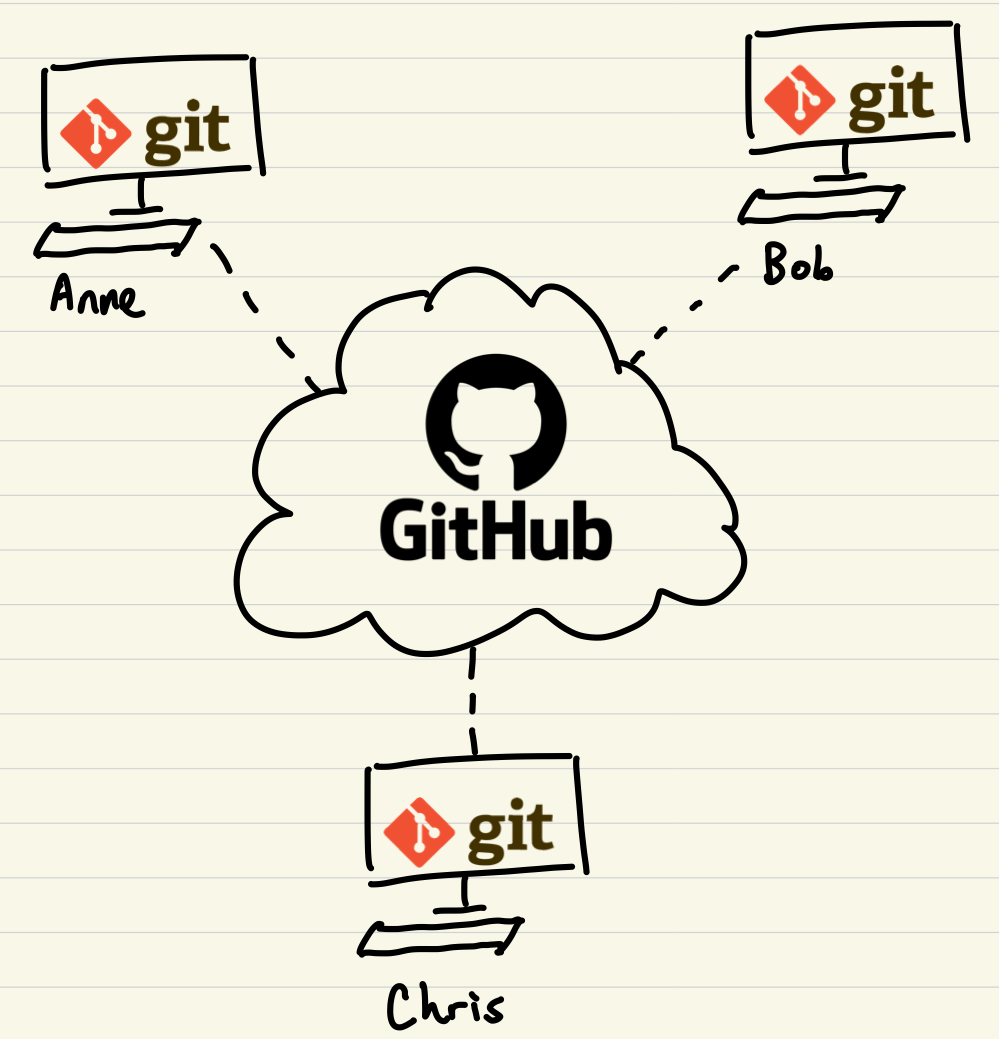
\includegraphics[width=10cm]{images/ch3-gitgithub.png}
\end{center}

\section{First time using Git}
\label{sec:gitfirst}

\textit{Covered in \href{https://www.youtube.com/watch?v=wQmFz-Ggxuo&list=PLjGmdnqrOKuYXiu7lgG5HW71jPEUd1XCm&index=4}{video 3 of the series}}
\vspace{6mm}

Let's just change \texttt{app/templates/views/index.pug} slightly so that we can make our first push to GitHub. Or if you are working on other projects, or you have made edits to \texttt{index.pug} or \texttt{abouts.pug} as instructed by previous chapters, you can just pick a random file or create a new one and make some edits.

\begin{lstlisting}[language=pug]
//- app/templates/views/index.pug
extends ../layouts/default

block content
	.container
		h1 Welcome to Static Web!
		br
		p A very cool website.
		p This web is made for tutorial purposes. //- ^new line
\end{lstlisting}

One very useful command - \texttt{git status} displays information about current situation, it might also contain some hints on which command(s) you should run to proceed.

\begin{lstlisting}[language=bash]
$ git status
On branch main
Your branch is up to date with 'origin/main'.

Changes not staged for commit:
  (use "git add <file>..." to update what will be committed)
  (use "git restore <file>..." to discard changes in working directory)
	modified:   app/templates/views/index.pug

no changes added to commit (use "git add" and/or "git commit -a")
\end{lstlisting}

\subsection*{First add}
So you can see it is prompting us to run \texttt{git add <file>}. Instead, I would prefer \texttt{git add .} As discussed in \cref{sec:dir}, \texttt{.} refers to the current directory. That means, we are including all the changes in the folder to be ready for a commit.

\begin{lstlisting}[language=bash]
$ git add .
\end{lstlisting}

Then, run \texttt{git status} again to asset the situation. The modified file should now be highlighted in green. (sadly you cannot see the green highlighting in \LaTeX)

\begin{lstlisting}[language=bash]
$ git status
On branch main
Your branch is up to date with 'origin/main'.

Changes to be committed:
  (use "git restore --staged <file>..." to unstage)
	modified:   app/templates/views/index.pug
\end{lstlisting}

\subsection*{First commit (and set up your name and email)}

Next step, we are now ready for commit. \texttt{git commit} seals and confirms our changes into one chunk, and adds a commit message. The \textbf{commit message} should be meaningful, summarising what we have achieved with these code changes.

\begin{lstlisting}[language=bash]
$ git commit -m "experimenting with git"
[main e7bc529] experimenting with git
Committer: KidProf <kidprof@KidProfs-MacBook-Air.local>
Your name and email addresses were configured automatically
...
git config --global --edit
git commit --amend --reset-author
1 file changed, 2 insertions(+), 1 deletion(-)
\end{lstlisting}

We got a problem here, our username and email do not match with the ones on GitHub. We need to \#1) change the default name and email on our device, and \#2) change the name and email for this particular commit.

Instead of the commands recommended automatically by Git, I recommend variants of those commands which are listed below, because these commands won't trigger the command line text editor to pop up. (see \cref{sec:vim})

Run the following two commands for \#1, replace the name and email with your own ones. Surround your name with double quotes if your name contains spaces.

\begin{lstlisting}[language=bash]
$ git config --global user.name KidProf
$ git config --global user.email kidprof@gmail.com
\end{lstlisting}

To verify, rerun those two commands but without the name and email, they should display your name and email as output.

\begin{lstlisting}[language=bash]
$ git config --global user.name
KidProf
$ git config --global user.email
kidprof@gmail.com
\end{lstlisting}

This command is for \#2.

\begin{lstlisting}[language=bash]
$ git config --amend --reset-author --no-edit
\end{lstlisting}

All set, now try running \texttt{git status} again. The warning is gone and Git is now prompting you to run the next command. 

\begin{lstlisting}[language=bash]
$ git status
On branch main
Your branch is ahead of 'origin/main' by 1 commit.
  (use "git push" to publish your local commits)

nothing to commit, working tree clean
\end{lstlisting}

\subsection*{First push}

Time to run \texttt{git push}, our last step. Except it might return an error.

\texttt{git push} uploads the commit from your local machine to GitHub. \textbf{Push} is another fancier word for upload.

\begin{lstlisting}[language=bash]
$ git push
fatal: The current branch main has no upstream branch.
To push the current branch and set the remote as upstream, use

    git push --set-upstream origin main
\end{lstlisting}

This one is quite an easy fix, just run the substitute command as instructed. You will need this whenever you are pushing a new branch to GitHub. \texttt{git push} should be sufficient for subsequent pushes.

\begin{lstlisting}[language=bash]
$ git push --set-upstream origin main
Enumerating objects: 11, done.
Counting objects: 100% (11/11), done.
Delta compression using up to 8 threads
Compressing objects: 100% (6/6), done.
Writing objects: 100% (6/6), 575 bytes | 575.00 KiB/s, done.
Total 6 (delta 3), reused 0 (delta 0), pack-reused 0
remote: Resolving deltas: 100% (3/3), completed with 3 local objects.
To github.com:KidProfMC/tutorial-website.git
\end{lstlisting}

\begin{center}
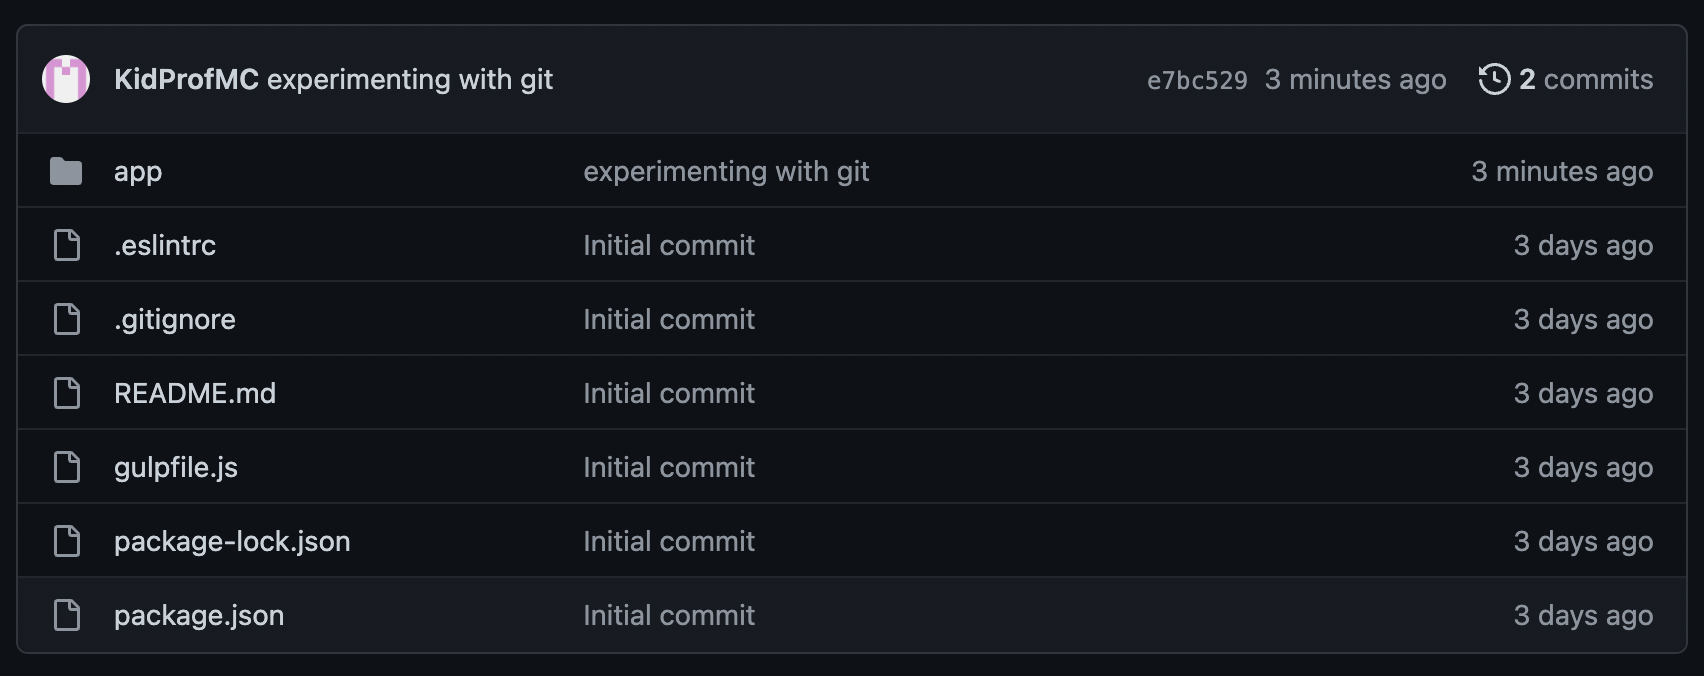
\includegraphics[width=12cm]{images/ch3-firstpushsuccess.png}
\end{center}

There you go, that is the first push. I will not list out the results of \texttt{git status} anymore in future sections, because they are taking too much space, but bear in mind running \texttt{git status} regularly is very useful.

\section{A typical day using Git}
\label{sec:gcmsg}

\textit{Covered in \href{https://www.youtube.com/watch?v=wQmFz-Ggxuo&list=PLjGmdnqrOKuYXiu7lgG5HW71jPEUd1XCm&index=4}{video 3 of the series}}
\vspace{6mm}

It is much more regular after the first push. You just need to remember three steps, add, commit and push.

\begin{lstlisting}[language=bash]
$ git add .
$ git commit -m "your message here"
$ git push
\end{lstlisting}

\texttt{git add} includes the changes you have made to be ready for the commit. 

\texttt{git commit} seals and confirms your changes into one chunk, and adds a commit message. The \textbf{commit message} should be meaningful, summarising what you have achieved with these code changes.

\texttt{git push} uploads the commit from your local machine to GitHub. \textbf{Push} is another fancier word for upload.
\vspace{6mm}

You should perform these three steps whenever you have made some progress on your code, as if it is a save button.

But there is an exception, you are not advised to push the code when your code failed to compile, because anybody else downloading the code would expect the code to run properly, at least for the parts of the code that are already finished in previous commits. But who cares when you are just working alone. :)

\subsection*{When do I have to set name and email like in the previous section?}

Every time you are using a new computer.

\subsection*{When do I have to add \texttt{--set-upstream} when pushing?}

Every time you are pushing a new branch to GitHub. You don't need to remember to do so because Git will reminds you anyways as shown in the previous section.

\section{Visualising}
\label{sec:sublime}
Git is a command line tool and is best used through the command line. Again, you will come across some situations where only command line is available (e.g. when accessing a remote server). 

However, it is acceptable if you just want to visualise the git commit history. Just don't run any commands using them. The following are two software recommended by me to do so. Sublime Merge looks nicer while Git Graph is embedded inside VS Code. 

\subsection*{Sublime Merge}

Download Sublime Merge by following \href{https://www.sublimemerge.com/}{this link}.\footnote{Link: \url{https://www.sublimemerge.com/}} It should be straightforward. 

After installing, open the repository folder. The commit history is displayed.

\begin{figure}[h]
\centering
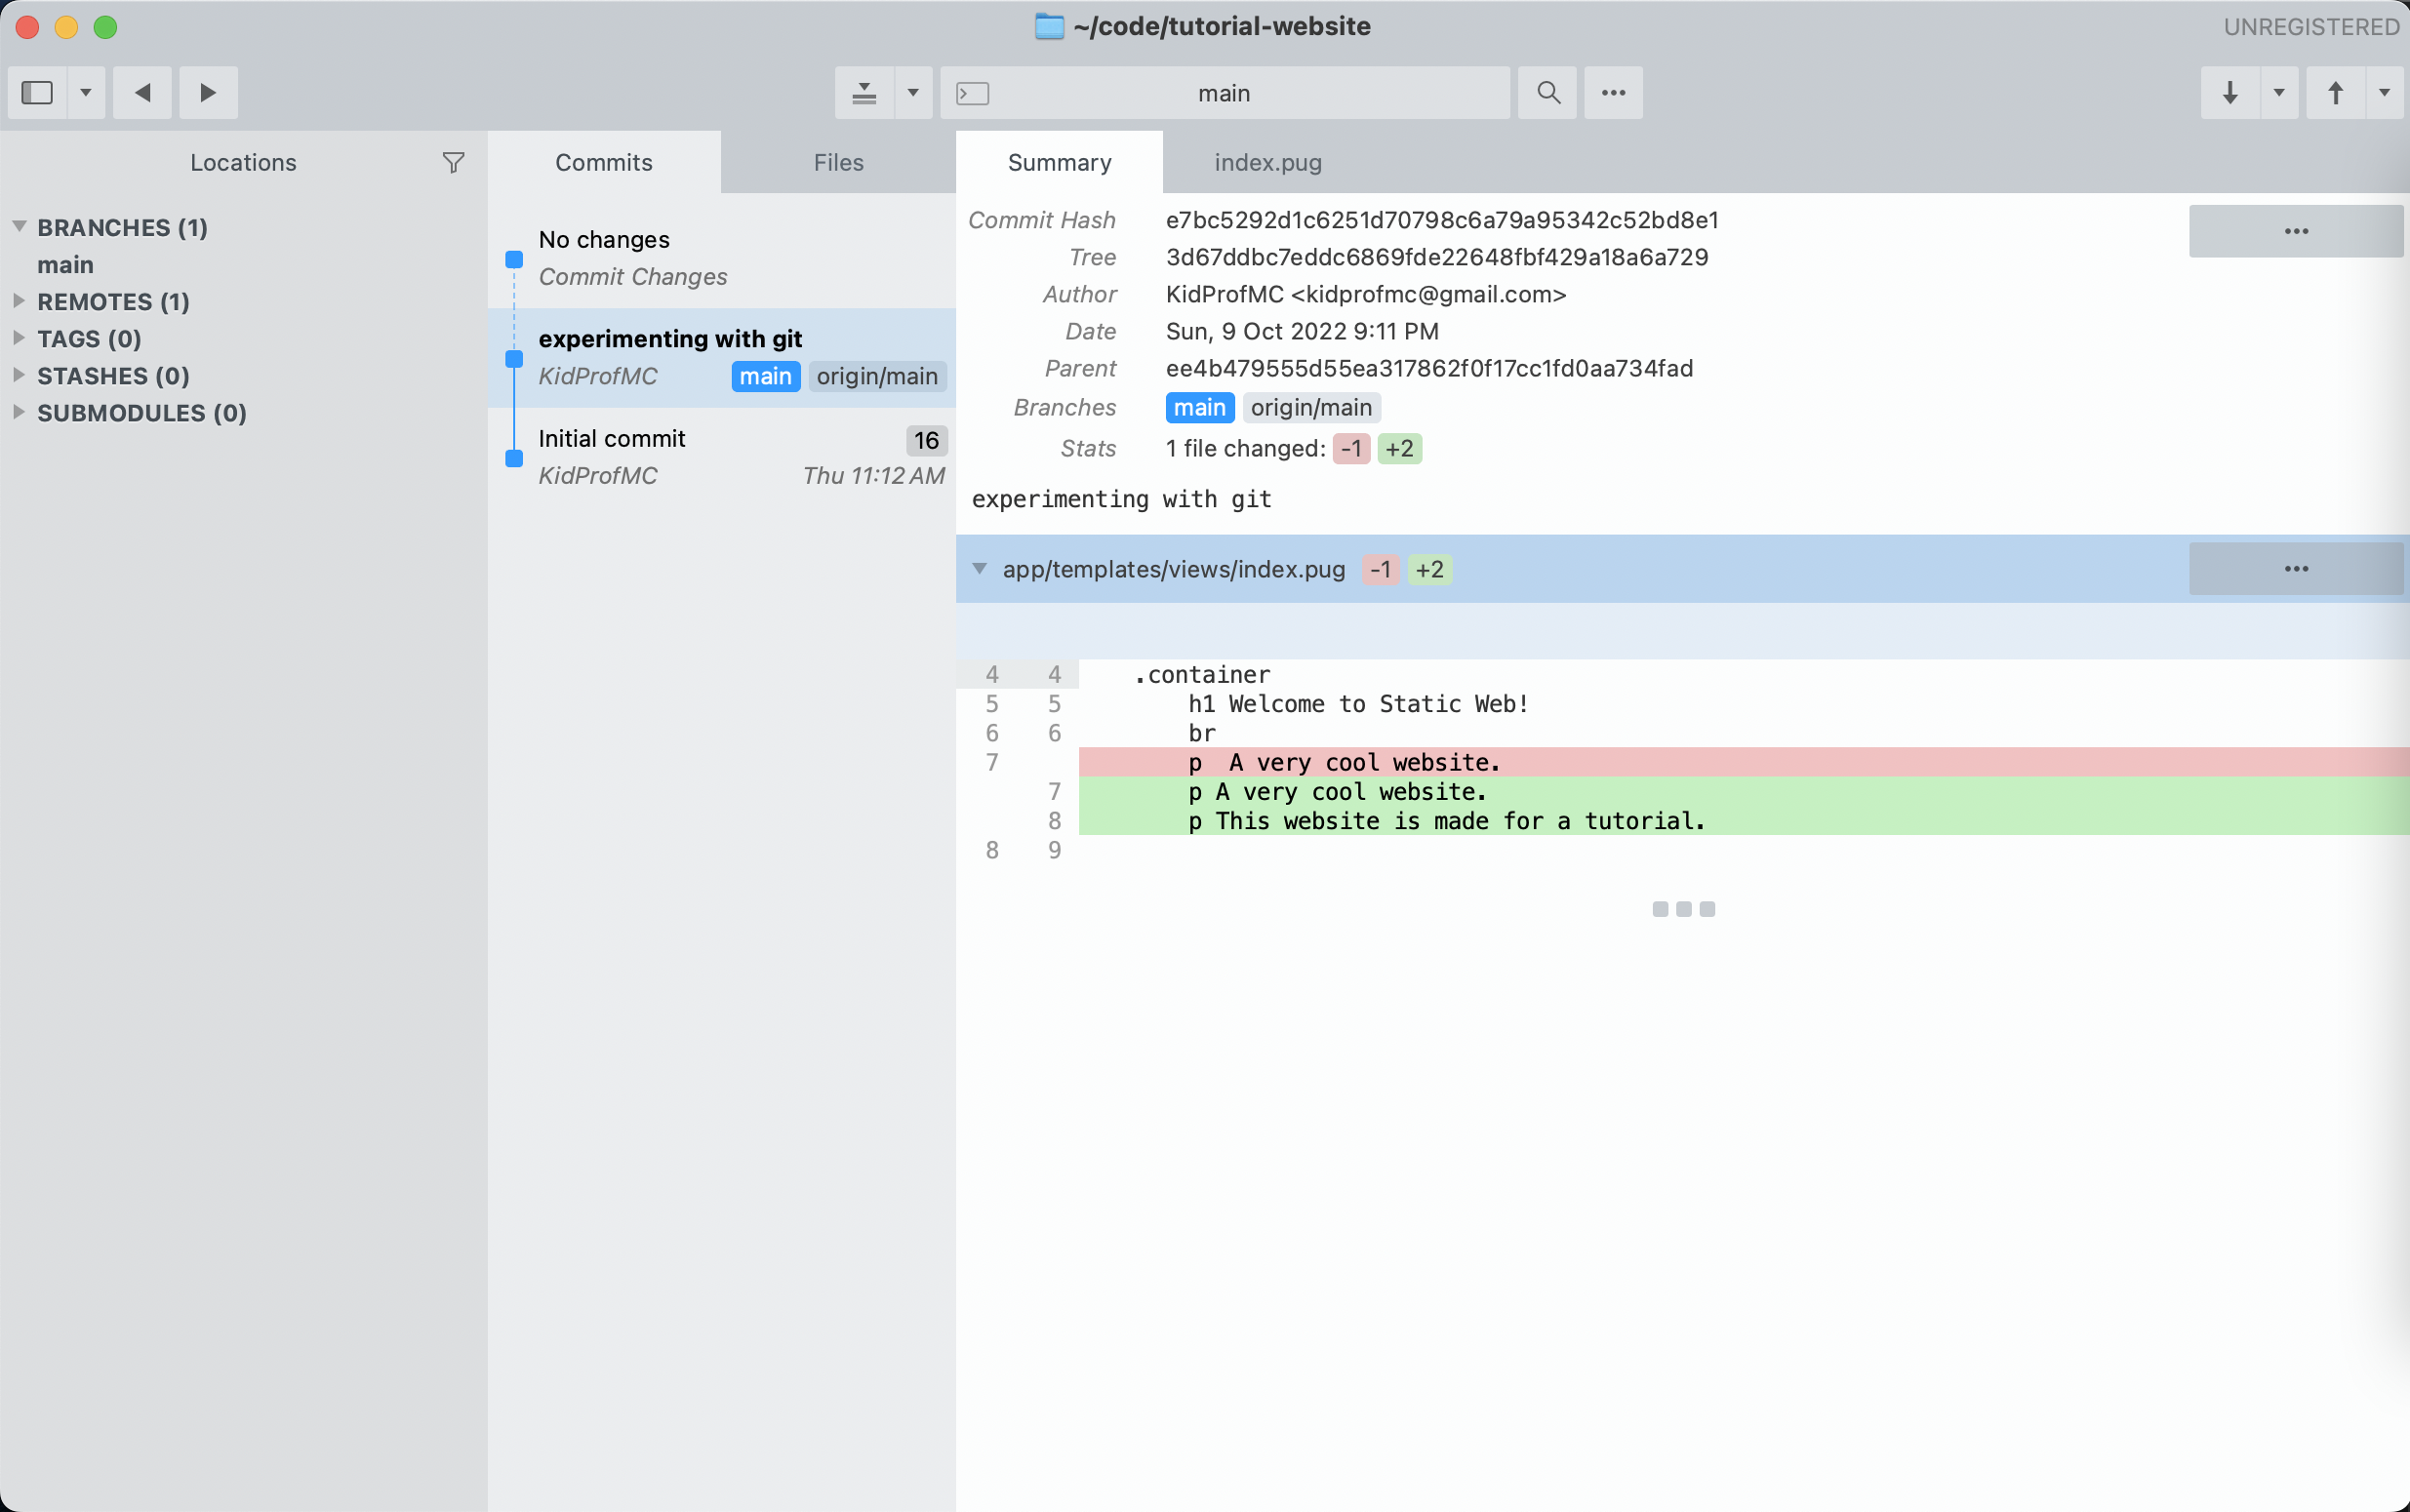
\includegraphics[width=15cm]{images/ch3-sublimemerge.png}
\caption{Sublime Merge showing our commit history throughout the chapter}
\end{figure}

\subsection*{Git Graph}

Git Graph is a VS Code extension, download it inside VS Code.

\begin{figure}[H]
\centering

\includegraphics[width=12cm]{images/ch3-gitgraph0.png}
\caption{Installation of Git Graph: Select extension on the menu on the left hand side, then search for Git Graph, then click install}
\end{figure}

Press \texttt{cmd+shift+P} or \texttt{ctrl+shift+P} to open the VS Code command bar, type \texttt{Git Graph: View Git Graph}

\begin{figure}[H]
\centering
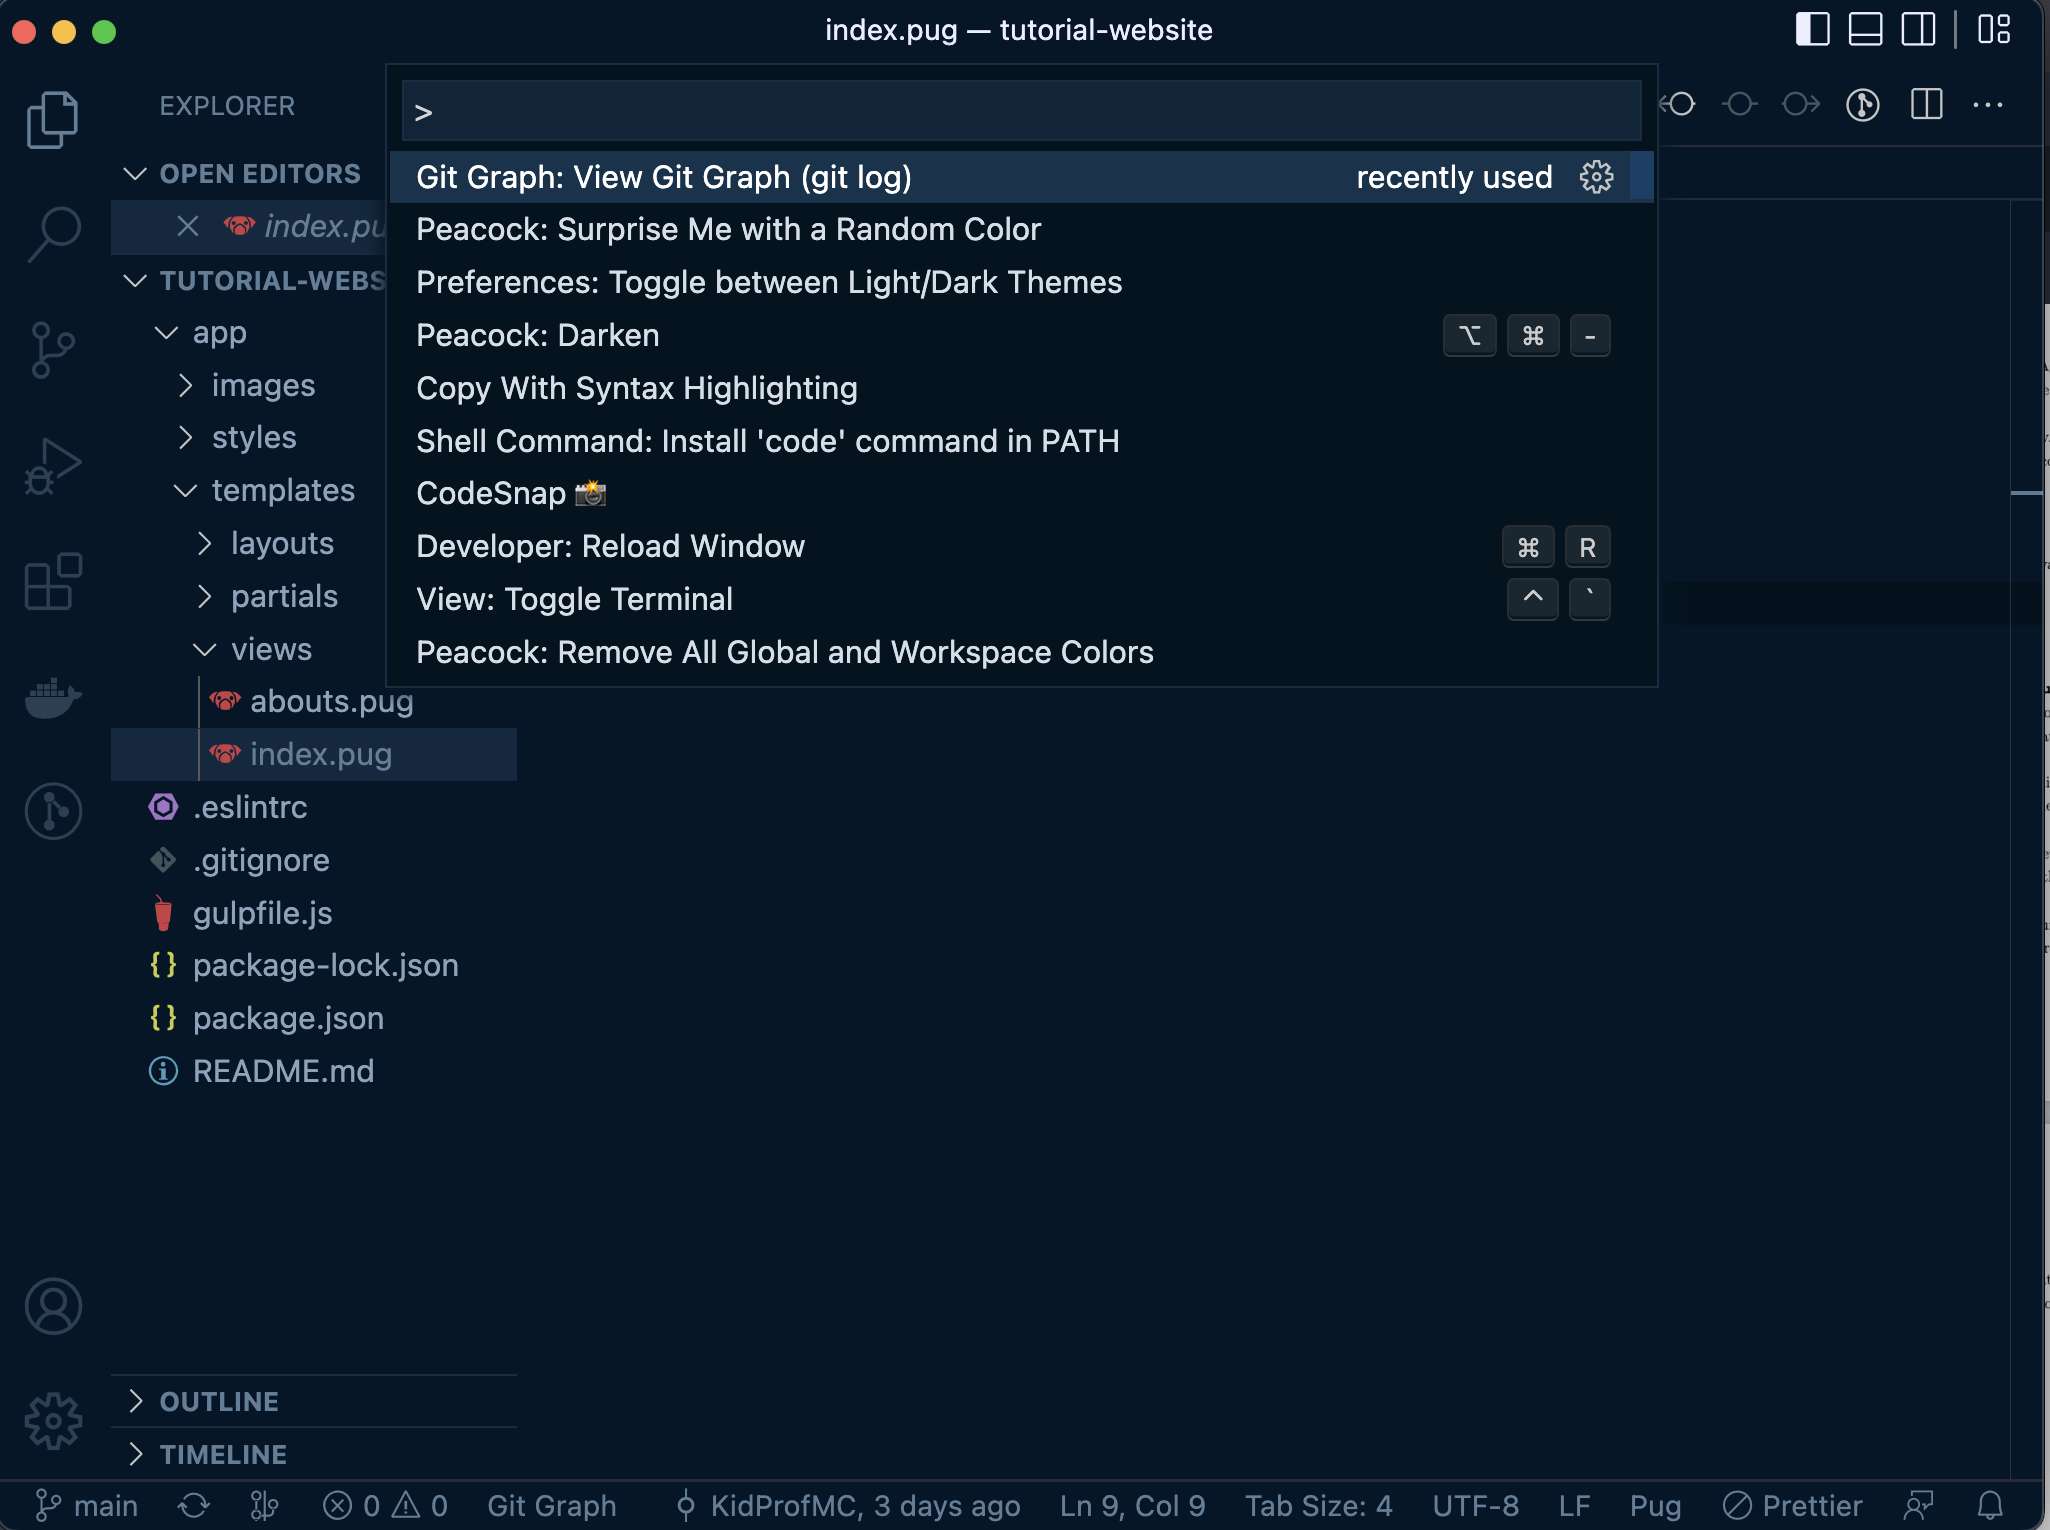
\includegraphics[width=12cm]{images/ch3-gitgraph1.png}
\caption{What is shown when \texttt{cmd+shift+P} or \texttt{ctrl+shift+P} is pressed}
\end{figure}

The commit history is displayed.

\begin{figure}[H]
\centering
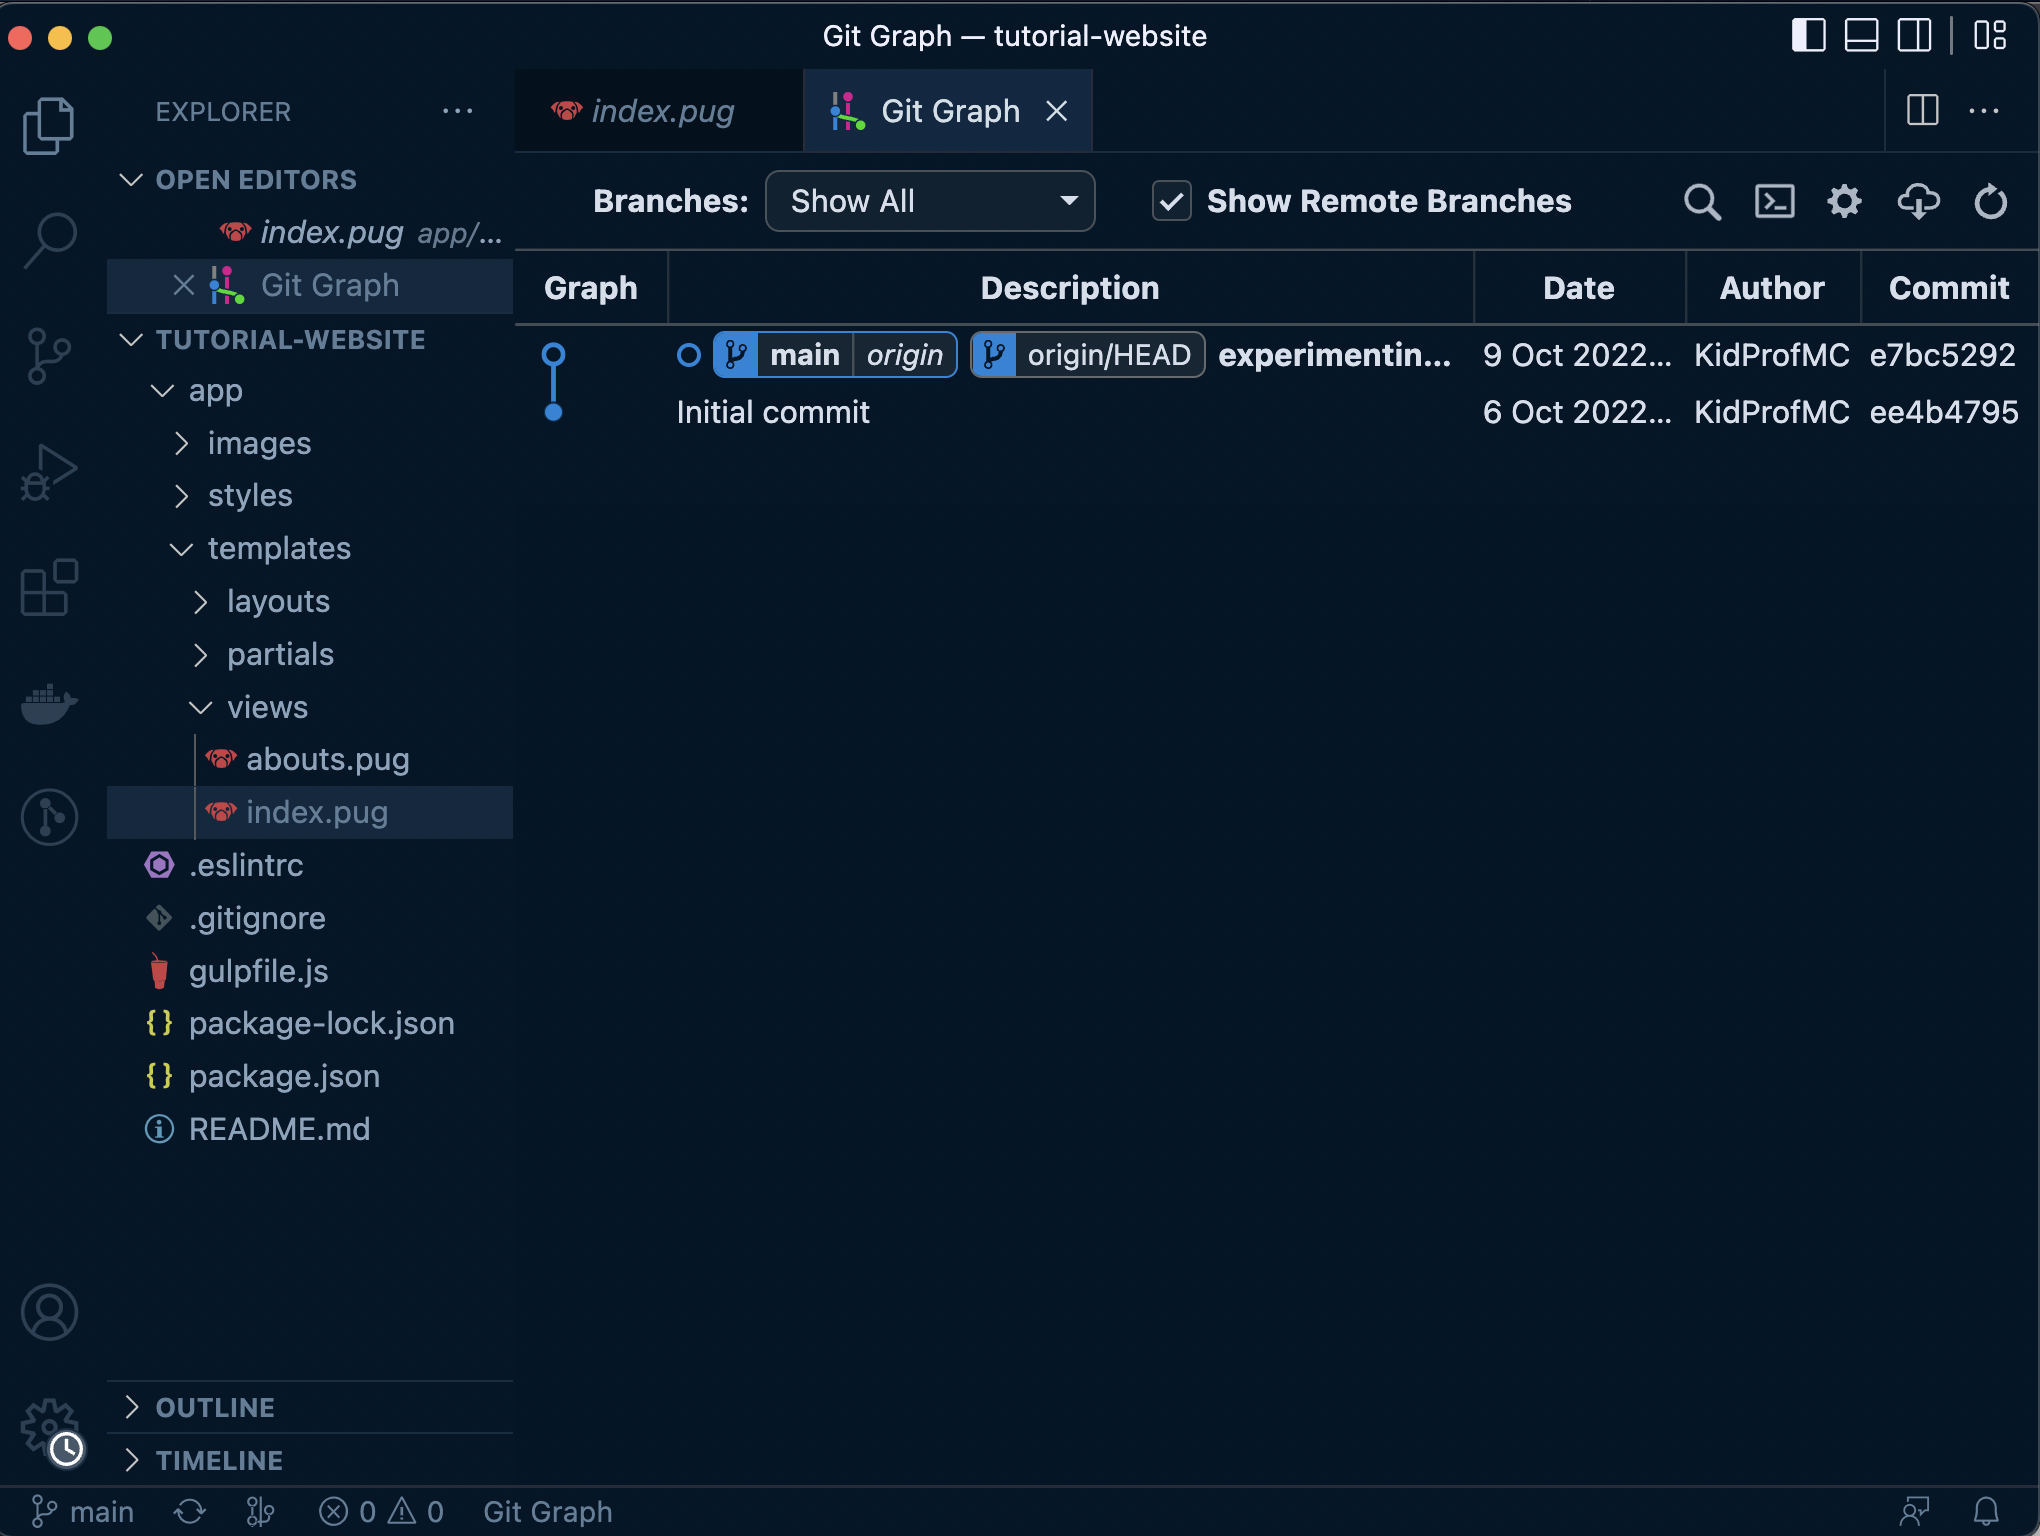
\includegraphics[width=12cm]{images/ch3-gitgraph2.png}
\caption{Git Graph showing our commit history throughout the chapter}
\end{figure}

\section{Something went wrong?}
\label{sec:gitpractice}

Anytime if you are unsure about what is happening with Git, \textbf{\texttt{git status}} is your best friend! It will display information about current situation, it might also contain some hints on which command(s) you need to run to get out of nasty situations.
\vspace{6mm}

If you added files that you don't want to push, and you have not committed, you can try \texttt{git restore <file>} to revert the changes for a particular file, or \texttt{git restore .} to revert all changes.

However, if you made some irreversible/ hard to reverse mistakes, which everybody will at some point in time. For example, you have made a commit at the wrong branch but haven't pushed, or you failed to fix a merge conflict (\cref{sec:mergeconflict}). 

In these cases, let's give up and use a cheesy way to fix it. Move all your code to another location so that you know what you have changed, clone the repository from GitHub again, then apply your changes to the new copy of the code, but with the mistakes fixed. It is completely fine, and sometimes the easiest way to do something.
\vspace{6mm}

Some of you who have learnt Git before may realise that there are other ways of using Git, mine is a more traditional command line approach, if you want to know why you can refer to \cref{sec:githubdesktop}.
\vspace{6mm}

If you will be working with others on the website you are creating using my template, it is highly recommended to read \cref{sec:git2} right after this. Else, you may carry on with the next chapter.
\section{Repositories}

\textit{Advanced}
\vspace{6mm}

Again, repository is a fancier name for project. Now we will look closely at this concept, and explain how to establish the relationship between your local code and the GitHub code.

\subsection{Creating a repository on GitHub}
\label{sec:gituploadgithub}

It is as simple as pressing a "New" button on the GitHub website, then fill in some simple details, such as your repository name and whether you would like your repository to be publicly visible or private, the decision is yours.

Then, you can either follow \cref{sec:gitinit} or \cref{sec:gitclone} to add your code in. 

You can add a \hyperref[sec:readme]{\texttt{README.md}} or \hyperref[sec:gitignore]{\texttt{.gitignore}}, the usage of such files will be explained in \cref{sec:readme} and \cref{sec:gitignore} respectively. However, it would make the repository no longer empty and you will have trouble following \cref{sec:gitinit}.

\subsection{Uploading existing local code to a new GitHub repository}
\label{sec:gitinit} 

\textit{\textbf{WARNING: } You can only do so when the GitHub repository is empty. If the GitHub repository is not empty, you will need to create a new one.}
\vspace{6mm}

Use \texttt{git init} in the folder with all your projects.

The use of \texttt{git branch -M main} is to change the name of the default branch from "master" to "main". A decision that GitHub made in 2020.\footnote{More info: \url{https://www.jumpingrivers.com/blog/git-moving-master-to-main/}}

Then follow your normal routine of adding and committing as above in \cref{sec:gcmsg}. There is a convention naming the first commit "init" or "initial commit".

Then \texttt{git remote add origin} is to establish the linkage between the local code and the GitHub repository, so that Git knows where to push to when you run \texttt{git push}, except for the first time, you need to run \texttt{git push -u origin main}.

\begin{lstlisting}[language=bash]
# KidProf in ~/code/your-project
$ git init

# No need to remember, copy from the GitHub docs
$ git branch -M main 

$ git add .
$ git commit -m "init"

# No need to remember, copy from the GitHub docs
$ git remote add origin git@github.com:KidProfMC/git-practice.git
$ git push -u origin main
\end{lstlisting}

\begin{figure}[h]
\centering
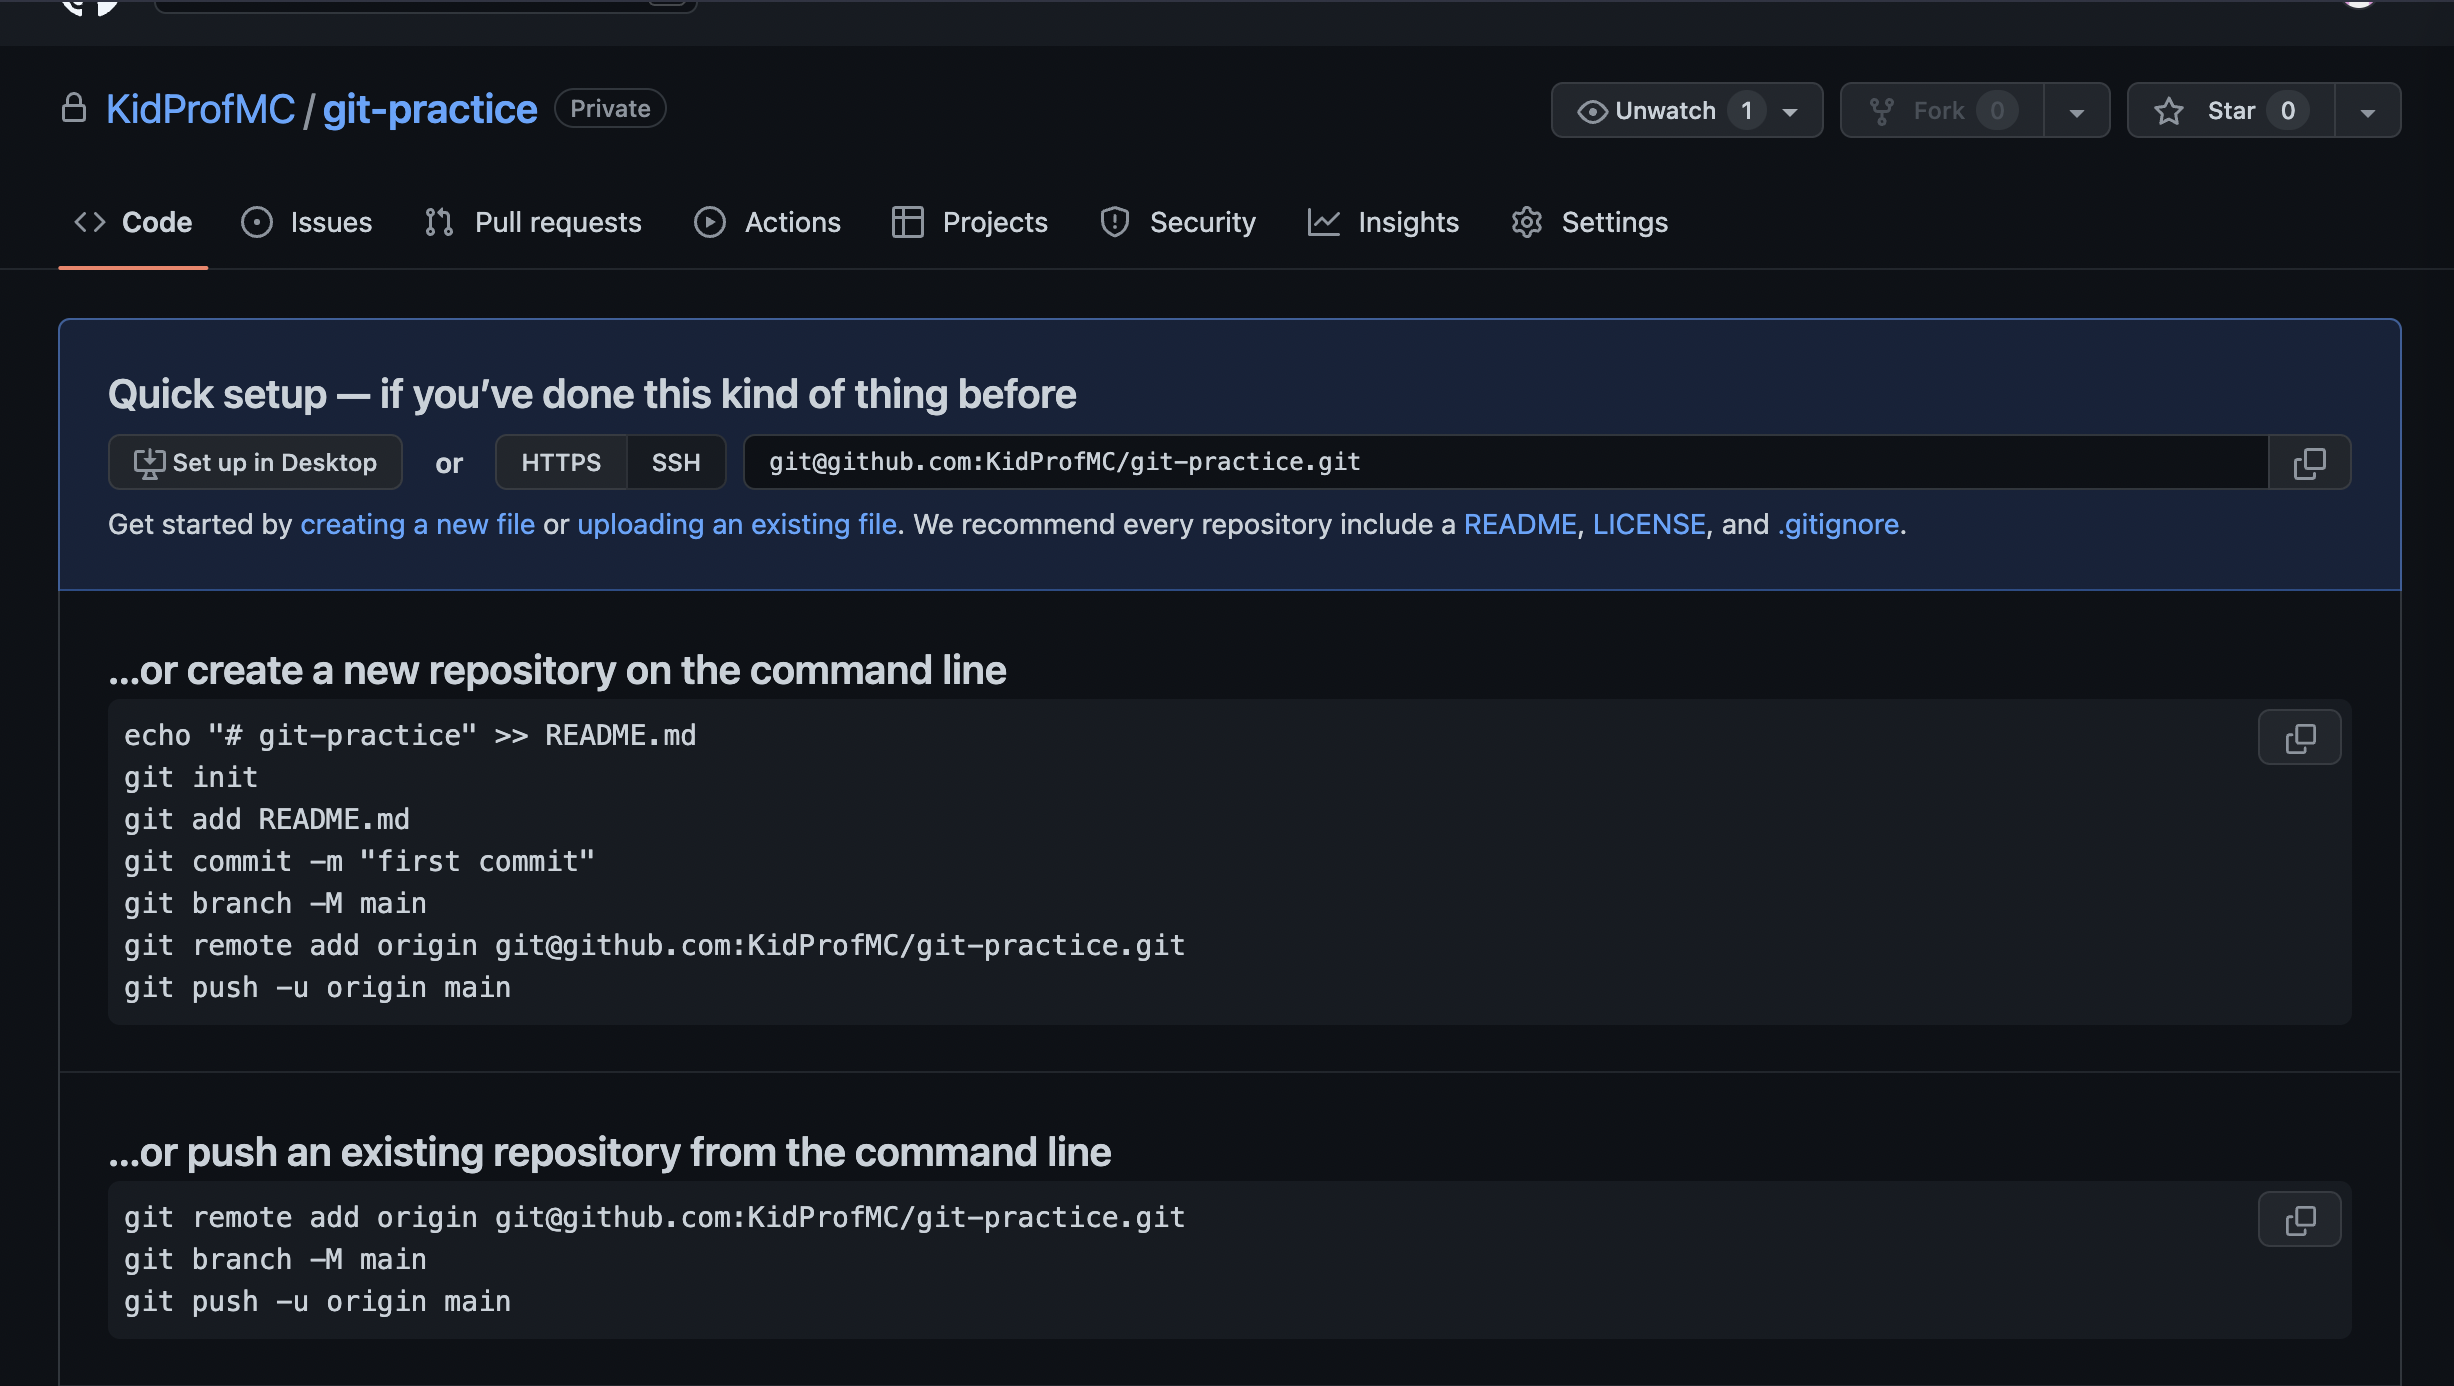
\includegraphics[width=15cm]{images/ch3-newrepocode.png}
\caption{The documentation on GitHub serves you well, we are following the upper part of the tutorial, remember to use SSH instead of HTTPS}
\end{figure}

\subsection{Downloading code from GitHub to local device}
\label{sec:gitclone}

Use \texttt{git clone} followed by the URL provided by GitHub, then a new folder with the repository name would be created with all the code inside. This is the method that we used in \cref{sec:install6}.

\begin{lstlisting}[language=bash]
# KidProf in ~/code
$ git clone git@github.com:KidProfMC/git-practice.git
$ cd git-practice
\end{lstlisting}

Then you can make updates on your code and push again.

If your repository is empty, you can move your code in, then perform the normal steps, we just have to name our commit "init" like in the previous section.

\begin{lstlisting}[language=bash]
$ git add .
$ git commit -m "init"
$ git push

# if git push returns an error, you can do:
$ git push --set-upstream origin main
\end{lstlisting}

\subsection{\texttt{.git} folder}

The \texttt{.git} folder contains everything that git needs to know to function normally, the commit history, the GitHub repository that it is linked to, etc.. If you remove the \texttt{.git} folder from your local device through the file explorer or finder (you need to enable the setting "show hidden files and folders"), or by the command \texttt{rm -rf .git}, all git information would be deleted. It might be useful if you are too confused and you want to reset everything related to Git.

\begin{table}[H]
    \centering
    \caption{Table of common Git commands in this chapter}
    \vspace{6mm}
    \begin{tabular}{|m{7em}|m{23em}|}
        \hline
        \textbf{Command} & 
        Description 
        \\ \hline \hline
        
        \texttt{git status} &
        Displays information about current situation, it might also contain some hints on which command(s) you should run to proceed. (\cref{sec:gcmsg})
        \\ \hline
        
        \texttt{git add .} &
        First step to push your code to GitHub - includes all the changes in the folder to be ready for a commit (\cref{sec:gcmsg})
        \\ \hline
        
        \texttt{git commit -m "message"} &
        Second step to push your code to GitHub - seals and confirms your changes into one chunk, and adds a commit message (\cref{sec:gcmsg})
        \\ \hline
        
        \texttt{git push} &
        Third step to push your code to GitHub - uploads the commit from your local machine to GitHub (\cref{sec:gcmsg})
        \\ \hline
        
        \texttt{git init} &
        Initialises a new Git repository in the current folder on your local machine (\cref{sec:gitinit})
        \\ \hline
        
        \texttt{git clone $<$url$>$} &
        Creates a new folder with the repository name would be created with all the code inside (\cref{sec:gitclone})
        \\ \hline
        
        
    \end{tabular}
\end{table}